\documentclass[letterpaper,12pt]{report}
\usepackage[utf8]{inputenc}
\usepackage[fleqn]{amsmath}
\usepackage{pgfplots}
\usepackage{tikz}
\usepackage{enumitem}
\usepackage{systeme}

\pgfplotsset{compat = newest}

% MACROS %
\newcommand{\evalmath}[1]{\pgfmathparse{#1}\pgfmathprintnumber{\pgfmathresult}}

\newcommand{\threetotwo}[4]{
  \begin{bmatrix}
    x_{#1} \\ y_{#1} \\
  \end{bmatrix} &=
  \begin{bmatrix}
    -0.5 & 1 & 0 \\
    -0.5 & 0 & 1 \\
  \end{bmatrix}
  \begin{bmatrix}
    #2 \\ #3 \\ #4 \\
  \end{bmatrix} =
  \begin{bmatrix}
    (-0.5 \cdot #2) + (1 \cdot #3) + (0 \cdot #4) \\
    (-0.5 \cdot #2) + (0 \cdot #3) + (1 \cdot #4) \\
  \end{bmatrix} =
  % \begin{bmatrix}
  %   (\evalmath{-0.5 * #2}) + (\evalmath{1 * #3}) + (\evalmath{0 * #4}) \\
  %   (\evalmath{-0.5 * #2}) + (\evalmath{0 * #3}) + (\evalmath{1 * #4}) \\
  % \end{bmatrix} =
  \begin{bmatrix}
    \evalmath{-0.5 * #2 + 1 * #3 + 0 * #4} \\
    \evalmath{-0.5 * #2 + 0 * #3 + 1 * #4} \\
  \end{bmatrix} \\
}

\newcommand{\threetotwov}[4]{
  \begin{bmatrix}
    x_{#1} \\ y_{#1} \\
  \end{bmatrix} &=
  \begin{bmatrix}
    -0.5 & 1 & 0 \\
    -0.5 & 0 & 1 \\
  \end{bmatrix}
  \begin{bmatrix}
    #2 \\ #3 \\ #4 \\
  \end{bmatrix} \\ &=
  \begin{bmatrix}
    (-0.5 \cdot #2) + (1 \cdot #3) + (0 \cdot #4) \\
    (-0.5 \cdot #2) + (0 \cdot #3) + (1 \cdot #4) \\
  \end{bmatrix} \\ &=
  \begin{bmatrix}
    \evalmath{-0.5 * #2 + 1 * #3 + 0 * #4} \\
    \evalmath{-0.5 * #2 + 0 * #3 + 1 * #4} \\
  \end{bmatrix} \\
}

\begin{document}
\begin{enumerate}[label=\alph*.]

\item 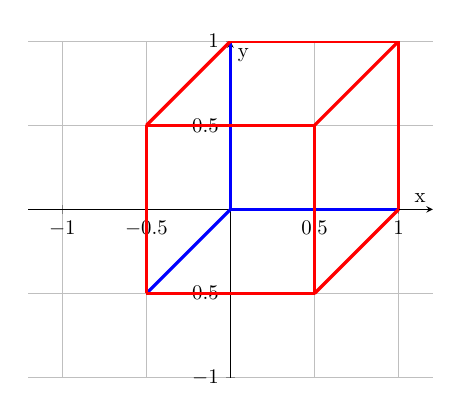
\begin{tikzpicture}[scale=0.75,baseline=(current bounding box.north)]
  \begin{axis}[
    axis lines=middle,
    axis equal,
    grid=both,
    xmin=-1,
    xmax=1,
    ymin=-1,
    ymax=1,
    xlabel=x,
    ylabel=y,
    every axis plot/.append style={ultra thick}
  ]
    \addplot[color=blue] coordinates{(0,0) (-0.5,-0.5)};
    \addplot[color=blue] coordinates{(0,0) (1,0)};
    \addplot[color=blue] coordinates{(0,0) (0,1)};

    \addplot[color=red] coordinates{(0,1) (-0.5,0.5)};
    \addplot[color=red] coordinates{(-0.5,-0.5) (-0.5,0.5)};
    \addplot[color=red] coordinates{(-0.5,-0.5) (0.5,-0.5)};
    \addplot[color=red] coordinates{(0.5,-0.5) (1,0)};

    \addplot[color=red] coordinates{(0.5,-0.5) (0.5,0.5)};
    \addplot[color=red] coordinates{(-0.5,0.5) (0.5,0.5)};
    \addplot[color=red] coordinates{(1,1) (0.5,0.5)};
    \addplot[color=red] coordinates{(1,1) (0,1)};
    \addplot[color=red] coordinates{(1,1) (1,0)};
  \end{axis}
\end{tikzpicture}

\begin{align*}
  \threetotwo{1}{0}{0}{0}
  \threetotwo{2}{1}{0}{0}
  \threetotwo{3}{0}{1}{0}
  \threetotwo{4}{0}{0}{1}
  \threetotwo{5}{1}{1}{0}
  \threetotwo{6}{0}{1}{1}
  \threetotwo{7}{1}{0}{1}
  \threetotwo{8}{1}{1}{1}
\end{align*}

\item \begin{minipage}[t]{.5\linewidth}
  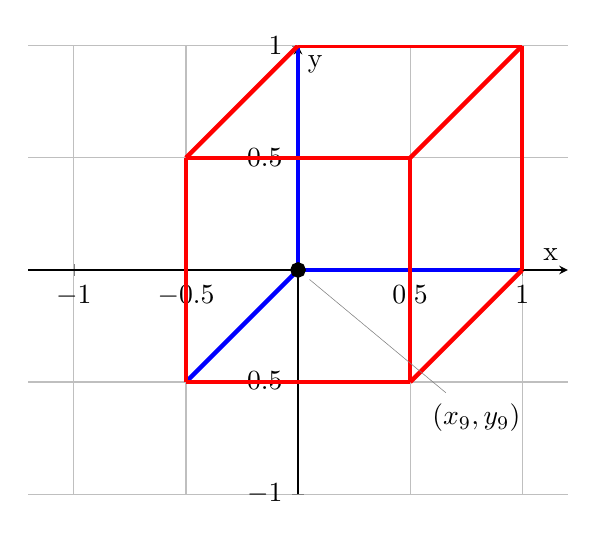
\begin{tikzpicture}[baseline=(current bounding box.north)]
    \begin{axis}[
      axis lines=middle,
      axis equal,
      grid=both,
      xmin=-1,
      xmax=1,
      ymin=-1,
      ymax=1,
      xlabel=x,
      ylabel=y,
      every axis plot/.append style={ultra thick}
    ]
      \addplot[color=blue] coordinates{(0,0) (-0.5,-0.5)};
      \addplot[color=blue] coordinates{(0,0) (1,0)};
      \addplot[color=blue] coordinates{(0,0) (0,1)};

      \addplot[color=red] coordinates{(0,1) (-0.5,0.5)};
      \addplot[color=red] coordinates{(-0.5,-0.5) (-0.5,0.5)};
      \addplot[color=red] coordinates{(-0.5,-0.5) (0.5,-0.5)};
      \addplot[color=red] coordinates{(0.5,-0.5) (1,0)};

      \addplot[color=red] coordinates{(0.5,-0.5) (0.5,0.5)};
      \addplot[color=red] coordinates{(-0.5,0.5) (0.5,0.5)};
      \addplot[color=red] coordinates{(1,1) (0.5,0.5)};
      \addplot[color=red] coordinates{(1,1) (0,1)};
      \addplot[color=red] coordinates{(1,1) (1,0)};

      \addplot[mark=*] coordinates {(0,0)} node[pin={[pin distance=2cm]315:{$(x_{9},y_{9})$}}]{} ;
    \end{axis}
  \end{tikzpicture}
\end{minipage}%
\begin{minipage}[t]{.5\linewidth}
  \begin{align*}
    \threetotwov{9}{1}{0.5}{0.5}
  \end{align*}
\end{minipage}

\item This problem can be expressed as
\begin{align*}
  \begin{bmatrix}
    -0.5 & 1 & 0 \\
    -0.5 & 0 & 1 \\
  \end{bmatrix}
  \begin{bmatrix}
    x_1 \\ x_2 \\ x_3 \\
  \end{bmatrix} =
  \begin{bmatrix}
    0 \\ 0 \\
  \end{bmatrix}
\end{align*}
It can then be turned into a system of equations:
\begin{align*}
  \systeme{
    -0.5x_1 + x_2 = 0,
    -0.5x_1 + x_3 = 0
  } \longrightarrow
  \systeme{
    -0.5x_1 + x_2 = 0,
    x_2 - x_3 = 0
  }
\end{align*}
Notice that $x_2 = x_3$. Let $x_2 = x_3 = r$. Solving for $x_1$,
\begin{align*}
  -0.5x_1 + r & = 0               \\
  -0.5x_1     & = -r              \\
  x_1         & = \frac{-r}{-0.5} \\
  x_1         & = \frac{r}{0.5}   \\
  x_1         & = 2r              \\
\end{align*}
Thus
\begin{align*}
  \begin{bmatrix}
  x_1 \\ x_2 \\ x_3 \\
  \end{bmatrix} =
  \begin{bmatrix}
  0 \\ 0 \\ 0 \\
  \end{bmatrix} +
  \begin{bmatrix}
  2r \\ r \\ r \\
  \end{bmatrix} = r
  \begin{bmatrix}
  2 \\ 1 \\ 1 \\
  \end{bmatrix}
\end{align*}

\end{enumerate}
\end{document}
